\section{Introduction}

This document is to summarise our experiments attempted to bias the seeding procedure of CC2538\cite{CC2538_Manual}.

The greatest difficulty is that details of how the seeding is done is not disclosed by the released documents from TI. The only descriptions in CC2538 User's Guide are:
\begin{quote}
...For the CC2538, when a random value is required, writing the SOC\_ADC\_RNDL register with random bits from the IF\_ADC in the RF receive path seeds the LFSR. To use this seeding method, first power on the radio. The radio must be placed in the infinite RX state to avoid possible sync detect in the RX state.The random bits from the IF\_ADC are read from the LSB position of the RF register RFCORE\_XREG\_RFRND. These bits should be concatenated over time to form the bytes needed for the RNG seed... This cannot be done while the radio is in use for normal tasks... (Section 16.2.2, CC2538 User's Guide)

...The RF Core can generate random bits. The chip should be in RX when generation of random bits is required. One must also make sure that the chip has been in RX long enough for the transients to have died out. A convenient way to do this is to wait for the RSSI-valid signal to go high. Single random bits from either the I or Q channel can be read from the RFRND register... (Section 23.12, CC2538 User's Guide)
\end{quote}

\Cref{CC2538_RFRND} shows the description of the crucial RFRND register in its manual.

\begin{figure}
\center
\caption{Description of RFRND from CC2538 User's Guide}
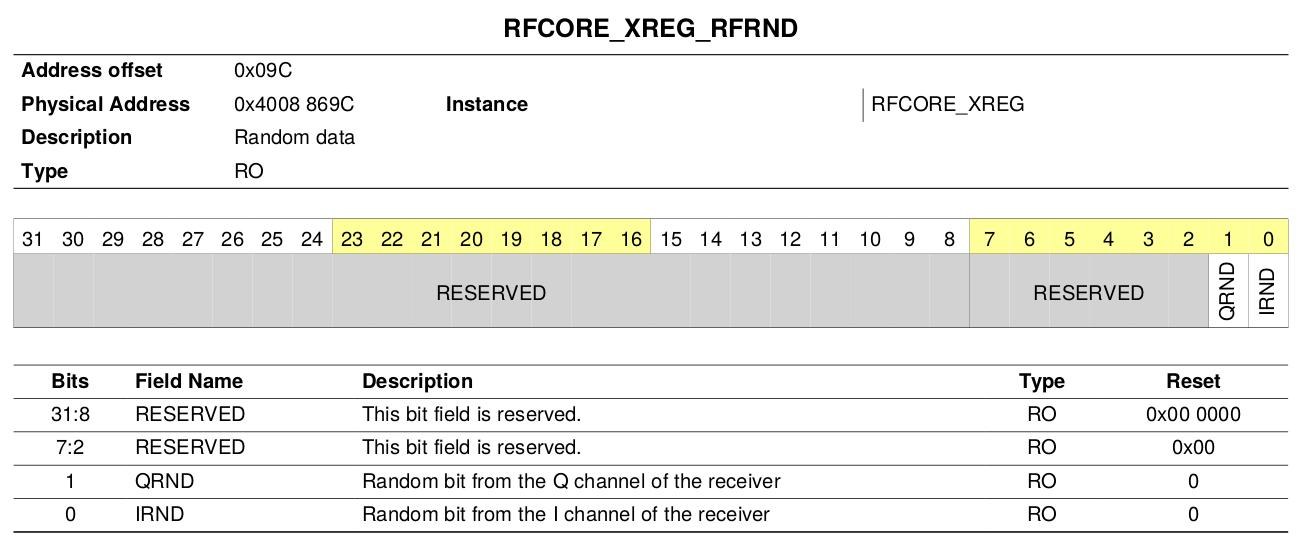
\includegraphics[width=\linewidth]{./figures/CC2538_RFRND.png}
\label{CC2538_RFRND}
\end{figure}

What we learned from the above descriptions are:
\begin{enumerate}
\item The random bits are derived from the IQ channels of IF\_ADC in the receive path, one bit at once, accessed through RFRND register.
\item The random bits are not available until the transients of IF\_ADC has died out.
\end{enumerate}

The above information seems to be good enough for developers to write drivers for this device. But from a security perspective, this method shed a light that the seed can be potentially affected by manipulating IF\_ADC through radio signals. However, there are several critical question that is not clear in the released documents:
\begin{enumerate}
\item How does IF\_ADC converts to a random bit?
\item Why infinite RX state is required?
\item Does RSSI play a role in the procedure? If yes, how?
\item What are the electronic characteristics? Including what is the IF, sample rate, etc.
\end{enumerate}

Without knowing the answers to these questions, we took two approaches to carry on the research:
\begin{enumerate}
\item Searching for related contents in the documents of product in the same series as they may shared the same design.
\item Black box experiments.
\end{enumerate}

CAUTION: Since the statements in this report are based on empirical document studies and black box experiments; thus they might not be accurate. As of writing this report, we have not yet successfully biased the seed.

\section{Related Documents Study}

CC2538, launched in May 2013, is not the first product that adopts the design of using RF to seed its PRNG, which is a 16-bit CRC16 LSFR register. The same design can trace back to one of its predecessor CC2430\cite{CC2430_Manual}, launched in 2007,  where a RNG failure has been explained by this blog\cite{CC2430Fail}.

In CC2430 User's Guide, we found the following instructions:
\begin{quote}
...When a true random value is required, the LFSR should be seeded by writing RNDL with random values from the IF\_ADC in the RF receive path. To use this seeding method, the radio must first be powered on by enabling voltage regulator as described in section 15.1. The radio should be placed in infinite TX\footnote{This is actually a typo. The RF needs to be in infinite RX state to use this seeding method.} state, to avoid possible sync detect in RX state. The random values from the IF\_ADC are read from the RF registers ADCTSTH and ADCTSTL (see page 196). The values read are used as the seed values to be written to the RNDL register as described above. Note that this can not be done while radio is in use for normal tasks... (Section 13.11.2.2, CC2430 User's Guide)
\end{quote}

We can see that CC2538 User's Guide basically inherited the same sentences, except that the seed is instead read from different registers, ADCTSTH and ADCTSTL. \Cref{CC2430_ADCTST} shows the detailed description of these registers in its manual.

\begin{figure}
\center
\caption{Description of ADCTSTH and ADCTSTL from CC2430 User's Guide}
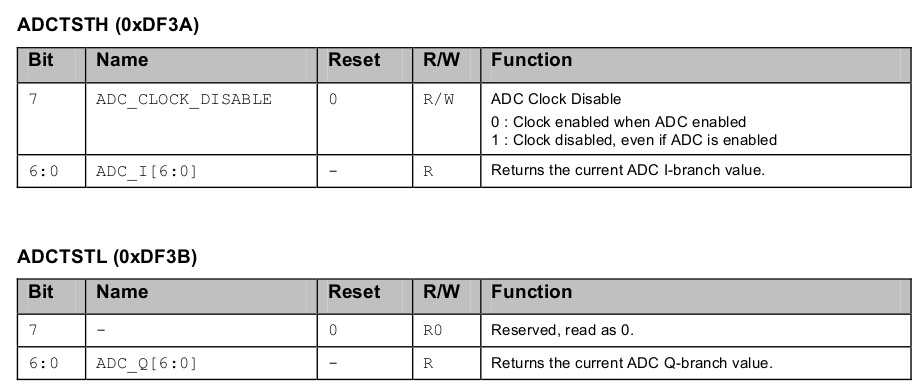
\includegraphics[width=\linewidth]{./figures/CC2430_ADCTST.png}
\label{CC2430_ADCTST}
\end{figure}

Comparing to CC2538, CC2430 User's Guide explains that the ADCs have resolution of 7-bits and one of their values is suggested to be directly used as the random seed. One thing might be worthy pointing out is that the entropy test in the blog post\cite{CC2430Fail} may have incorrectly interpreted these 7-bits readings as a byte, even though it does not change the fact that such seed is strongly biased.

CC2430 also disclosed more details about its RF. \Cref{CC2430_RF} provides an overview of its RF design, which is relatively classic. We can see that the random seed from IF\_ADC is indeed the output of mixer after band pass filter and AGC, where LO is implemented by the Frequency Synthesiser.

\begin{figure}
\center
\caption{Radio and Demodulator of CC2430 from CC2430 User's Guide}
\begin{subfigure}{\linewidth}
%	\subcaption{Block Diagram of Radio Module from CC2430 User's Guide}
	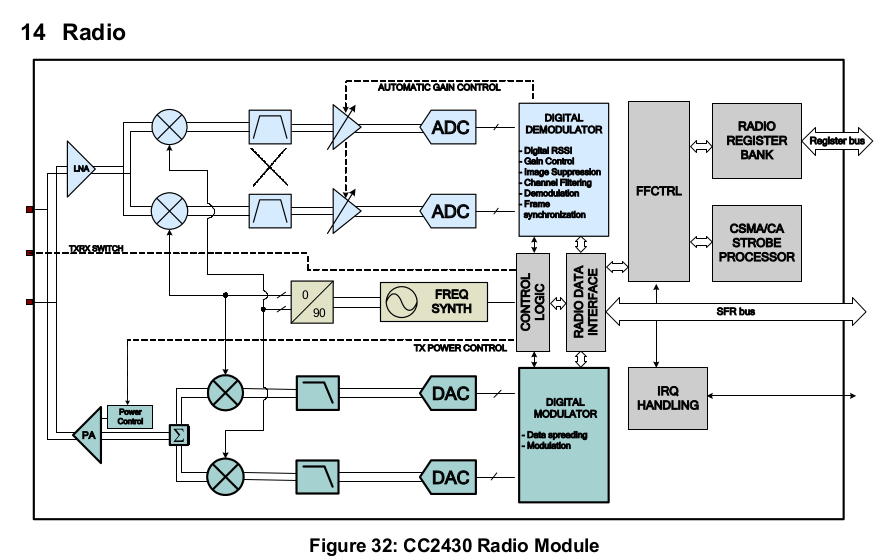
\includegraphics[width=\linewidth]{./figures/CC2430_Radio.png}
\end{subfigure}

\begin{subfigure}{\linewidth}
%	\subcaption{Block Diagram of Demodulator from CC2430 User's Guide}
	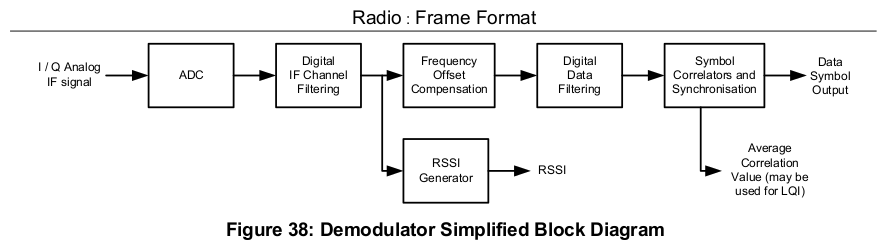
\includegraphics[width=\linewidth]{./figures/CC2430_Demodulator.png}
\end{subfigure}
\label{CC2430_RF}
\end{figure}

The CC253X and CC2540/41 series\cite{CC253X_Manual} is another sibling of CC2538 launched in April 2009. This series also inherited the similar RNG design from CC2430, using a CRC16 register as PRNG seeded by IF\_ADC.

\begin{quote}
...For the CC253x, when a random value is required, the LFSR should be seeded by writing RNDL with random bits from the IF\_ADC in the RF receive path. To use this seeding method, the radio must first be powered on. The radio should be placed in the infinite RX state to avoid possible sync detect in the RX state. The random bits from the IF\_ADC are read from the least-significant bit position of the RF register RFRND. These bits should be concatenated over time to form the bytes needed for the random-number-
generator seed... (Section 14.2.2, CC253X, CC2540/41 User's Guide)
\end{quote}

\Cref{CC253X_RFRND} shows the RFRND register for CC253X.

\begin{figure}
\center
\caption{Description of RFRND from CC253X, CC2540/41 User's Guide}
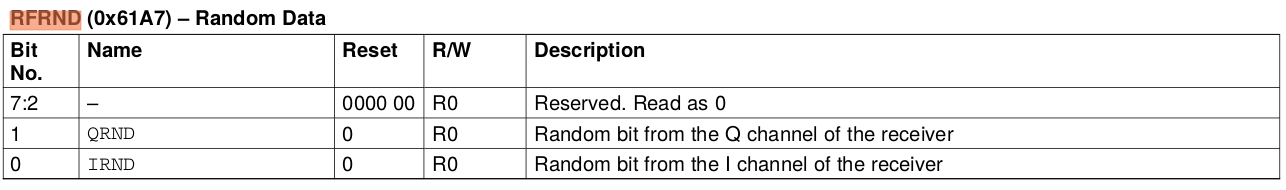
\includegraphics[width=\linewidth]{./figures/CC253X_RFRND.png}
\label{CC253X_RFRND}
\end{figure}

Further inspecting the documents, we realised that CC253X and CC2538 reported exactly identical seeding result in their manuals, as shown in \Cref{CC2538_CC253X_SeedComparison}. This suggests that CC2538 and CC253X are likely used the same RF module.

\begin{figure}
\center
\caption{Seeding Result for CC253X and CC2538}
\begin{subfigure}{0.8\linewidth}
	\subcaption{Seeding Result from CC253X,CC2540/41 User's Guide}
	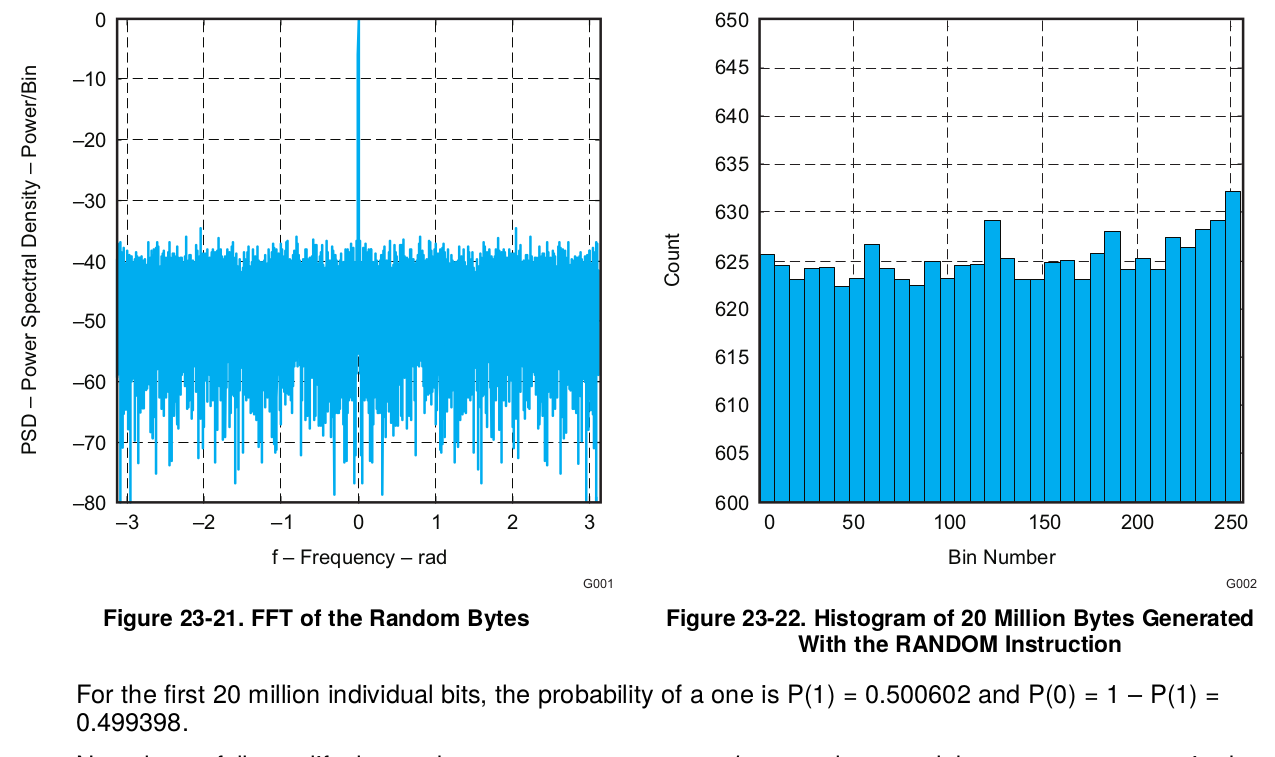
\includegraphics[width=\linewidth]{./figures/CC253X_Seed.png}
\end{subfigure}

\begin{subfigure}{0.8\linewidth}
	\center
	\subcaption{Seeding Result from CC2538 User's Guide}
	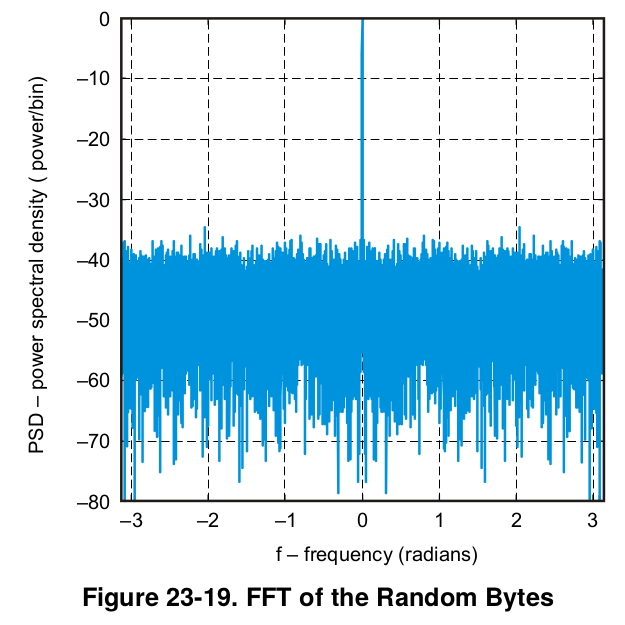
\includegraphics[width=0.55\linewidth]{./figures/CC2538_Seed1.png}
	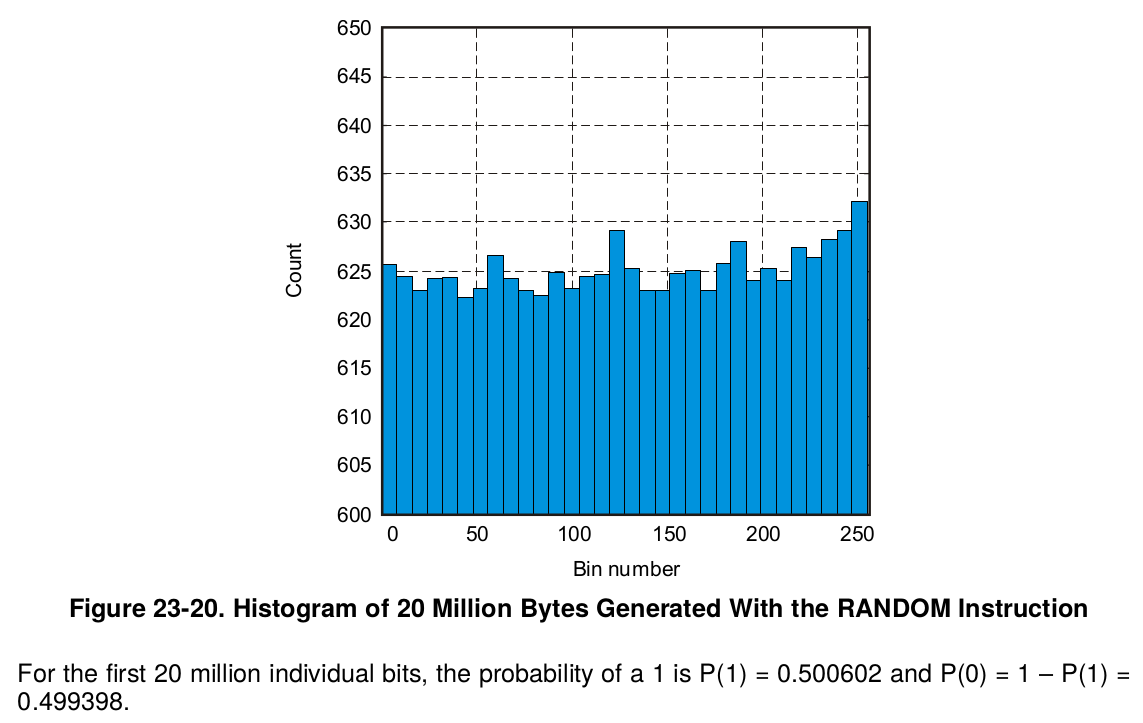
\includegraphics[width=\linewidth]{./figures/CC2538_Seed2.png}
\end{subfigure}
\label{CC2538_CC253X_SeedComparison}
\end{figure}

But the problem remains that neither CC253X nor CC2538 explained how IF\_ADC is translated to the output of RFRND. Nevertheless, we found the following statement in the instructions for CC2541 running in proprietary mode:
\begin{quote}
...For seeding the pseudo-random number generator and for tasks where higher entropy of the random numbers is needed, the radio can be used as a true-random generator. The register RFRND provides access to the least-significant bits of the radio ADC, which is random when noise is received.... (Section 25.10, CC253X, CC2540/41 User's Guide)
\label{CC2540 RND}
\end{quote}

This instruction explicitly explains that RFRND actually reads the least significant bit of IF\_ADC.

Given the similarities of these SoCs, we suspect RFRND in CC2538 is also  the least significant bit from its IF\_ADC.

In summary, we suspect the following undisclosed characteristics of CC2538:
\begin{enumerate}
\item CC2538 has a similar classical RF circuit design as of CC2430.
\item CC2538 has exactly the same RF specifications of CC253X.
\item RFRND is implemented as the least significant bit from IF\_ADC as of CC2541.
\end{enumerate}

We based our further experiments on these assumptions.

\section{Contiki Driver}

Contiki release-3.0 exactly followed the instructions in CC2538 User's Guide. Generally speaking, it performed the following operations during seeding the CRC16 PRNG:
\begin{enumerate}
\item Turns on the CRC16 PRNG and enables clock for RF.
\item Sets RF to infinite RX state. This will take effect on next RF start.
\item Turns on RF. This also triggers the Frequency Synthesiser to recalibrate.
\item Waits for transients to die out by checking RSSI validity. This also implies that the Frequency Synthesiser is calibrated.
\item Reads 16 bits from RFRND.
\item Set PRNG seed by values from RFRND.
\item Turn off RF. It will be turned on again later for normal operation.
\end{enumerate}

The original source code is listed in \Cref{ContikiRngDriver}. A coding mistake caused the least significant bit (the 16th bit) to be constantly 0. We have fixed this bug during our experiments.

\section{Randomness Test}
We first tested the randomness of CC2538's seeding method using the NIST Statistical Test Suite\cite{NistTestSuite}. 

The test is performed on 13738816 bits recorded by looping Contiki driver, with each loop reads out 16 bits from RFRND. Since each read to RFRND returns only 1 bit, we concatenated the result into one bit stream. The random bit stream has passed all the tests with $P(0) = 49.9380\%$, which consists to the result of the manual. The full test report is listed in \Cref{NistTestReport}.
%
%\section{Extending Seed Length}
%
%CC2538 User's Guide suggests that RFRND is used only to seed the CRC16 PRNG and thus only 16 bits are needed. We modified the code to continuously read out 8096 bits from RFRND, which is not an expected legal behaviour according in the manual. The seed is printed through UART to a Linux terminal.
%
%\begin{figure}[ht!]
%\center
%\caption{Reading 8096 bits from CC2538 RFRND}
%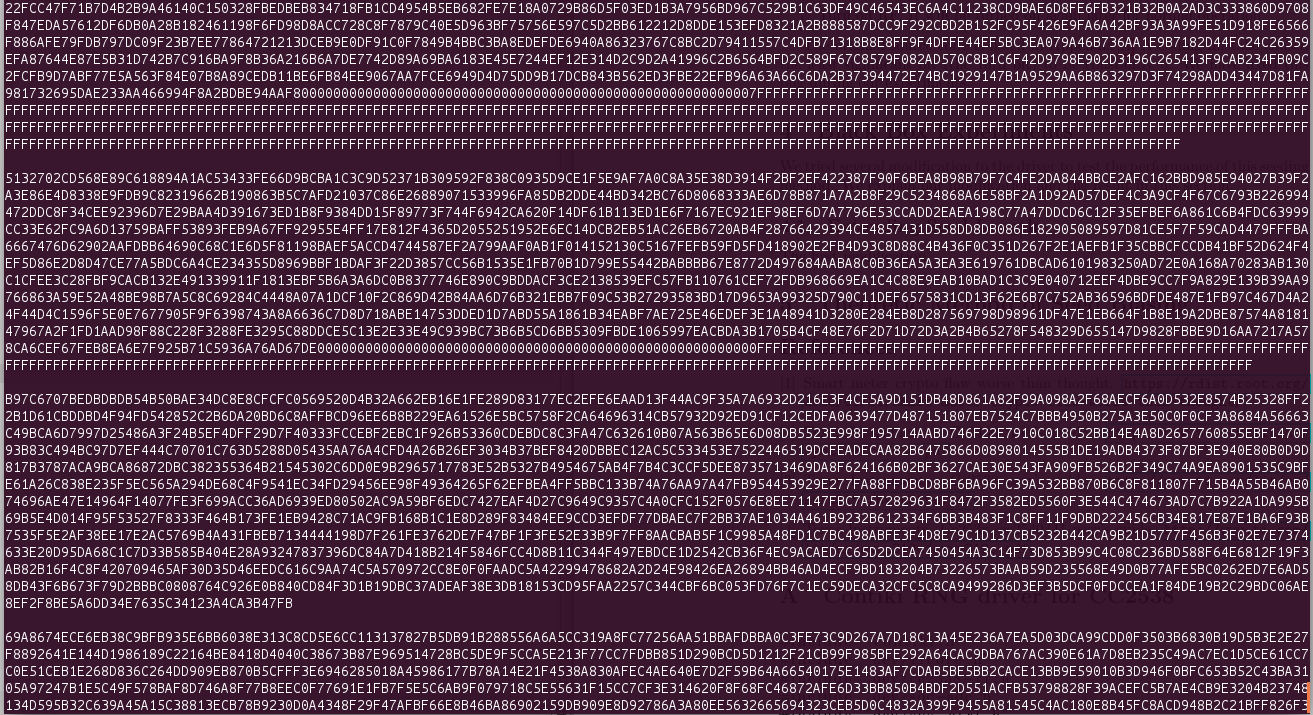
\includegraphics[width=\linewidth]{./figures/SeedExtend.png}
%\label{RFRND8096}
%\end{figure}
%
%\Cref{RFRND8096} shows part of the result. Occasionally RFRND falls into a broken state after some readings.  Under such state, it outputs purely 0 or 1 with  a potential flip after the beginning few bits as shown in \Cref{RFRND8096}. Extending the length of seed to 32768 bits, we realised the error happens in every seeding procedure.

\section{Theoretical Method of Seed Biasing}

The description of the RFRND implementation on CC2540 (\Cref{CC2540 RND}) gave a hint that CC2538 may also have used the least significant bit of IF\_ADC output as  a random bit. The output of IF\_ADC is effectively the analogue output of the mixer converted to digital.

\subsection{About Mixer and RFRND}

Mixer is a electric component used to convert a signal to lower or higher frequencies. A typical mixer is illustrated in \Cref{mixer}.

\begin{figure}
\center
\caption{Mixer Illustration}

\includegraphics[width=0.5\linewidth]{figures/mixer.png}
\label{mixer}
\end{figure}

The mixer takes two analogue input, RF and LO, and outputs IF which is the mixture of RF and LO. In our specific case,
\begin{itemize}
\item RF is the signal received by antenna amplified by LNA\footnote{Low Noise Amplifier}. For 802.15.4 communication, RF frequency $f_{R}$ is specified by 802.15.4 standard\cite{802154_Standard}:
\begin{eqnarray}
f_{R} = 2405 + 5(k-11) [MHz] && k \in [11, 26]
\end{eqnarray}
where $k$ is the selectable channel number.

\item LO is a signal generated by the frequency synthesiser. The exact frequency of LO, denote as $f_{L}$, is adjusted according to required IF frequency.
\end{itemize}

Typically, the mixer can be implemented as the product of RF and LO. Denote the signals of RF and LO as $\cos(\omega_{R}t + \theta_{R})$ and $\cos(\omega_{L}t)$ respectively, the IF output is:

\begin{equation} \label{IF}
\begin{split}
A_{R}\cos(\omega_{R}t)A_{L}\cos(\omega_{L}t) &= {\frac{A_{R}A_{L}}{2}}\cos((\omega_{R} + \omega_{L})t) + {\frac{A_{R}A_{L}}{2}}\cos((\omega_{R} - \omega_{L})t)
\end{split}
\end{equation} 

where $t$ is time and $\omega_i = 2{\pi}f_i$.

\Cref{IF} implies that there are two signals outputted by IF, of one at frequency $(\omega_{R} + \omega_{L})$ and the other $(\omega_{R} - \omega_{L})$. In RF receiving path,  the mixer down converts the high frequency RF signal to low frequency signal that can be processed by local components; thus the signal at the higher frequency is then filtered, e.g. the band pass filters in both I and Q channels in \Cref{CC2430_RF}. So the input to IF\_ADC is:
\begin{equation}
x(t) = A'\cos((\omega_{R} - \omega_{L})t)
\end{equation}
where $A'$ is the amplitude adjusted by AGC. 

The random bit $b$ of RFRND can then be represented as:
\begin{equation} \label{RFRND}
b = \lfloor{x(t)} \mod 2V_0 \rfloor = \lfloor{A'\cos((\omega_{R} - \omega_{L})t) \mod 2V_0 }\rfloor
\end{equation}

where $V_0$ is the amount of measurement represented by the least significant bit of the ADC. The actual value of $b$ may be $\pm 1$ according to how ADC is implemented. Notice that \Cref{RFRND} does not take noise into account.

\subsection{Noise}

In real world deployment, the RF input is inevitably affected by several noise sources, include:

\begin{itemize}
\item Environmental radio noise.
\item Radio noise induced by the electronic system itself.
\item Approximation error within the system.
\end{itemize}

Denote $N(t)$ to be the noise in the input to IF\_ADC, \Cref{RFRND} should be rewritten as:

\begin{equation} \label{RFRND_noise}
\begin{split}
b &= \lfloor{(A'\cos((\omega_{R} - \omega_{L})t) + N(t) )\mod 2V_0 }\rfloor \\
&= \lfloor{(A'\cos((\omega_{R} - \omega_{L})t) \mod 2V_0 + N(t) \mod 2V_0 }\rfloor
\end{split}
\end{equation}

\Cref{RFRND_noise} suggests that any noise above $V_0$ may flip the bit $b$. According to CC2538 data sheet\cite{CC2538_Datasheet}, the RF receiver can be sensitive down to radio signals of $-97$dBm, whereas in our testing office environment, i.e. with multiple electronic devices and strong WiFi signal presented, the environmental noise easily exceeds this level. By nature noise is practically difficult to control, this poses a great difficulty when trying to manipulate the RFRND output.

\subsection{Affection of Jamming Signal}

When generating RF signal to affect $b$ in \Cref{RFRND_noise}, the adversary can be considered to have full control on RF frequency $\omega_{R}$ and potentially partial control of $A'$ by adjusting $A_{R}$. Since RFRND only outputs one bit at once, the options are either:
\begin{itemize}
\item Bias RFRND to $0$. 
\item Bias RFRND to $1$.
\end{itemize}

Two methods are considered to bias RFRND to $0$:
\begin{enumerate}
	\item Cancel, or mitigate, $N(t)$ by RF.  
	\item Ground the input of IF\_ADC. 
\end{enumerate}

These methods seems impractical in our circumstance given the high sensitivity of the device. The first method fails due to the unpredictability of $N(t)$. For the second method, we tried to connect the antenna to the GND pin on the board it does not seem to have a effect neither.

On the other hand, biasing RFRND to $1$ seems more practical. Ideally, when an input voltage equal or higher than the maximum allowance is given, the ADC will output a fixed maximum value $V_{max}$ which the least significant bit is likely to be $1$. 

The idea is therefore to send a jamming signal that is strong enough to saturate ADC. We expect IF\_ADC to output its maximum value which normally has a least significant bit of $1$.


